%=====================��=======��==============================
\documentclass[a4paper, 12pt]{article}
%======================Include Packages========================
\usepackage{amsfonts}
\usepackage{amsmath}
\usepackage{amsthm} %to use \proof environment
\usepackage{amssymb} %to use \because and \therefore
% \usepackage{algorithm}
\usepackage[ruled,linesnumberedhidden]{algorithm2e} %��natbib��������
\usepackage{authblk}
% \usepackage{algpseudocode}
%\usepackage{bibliography}
%\usepackage{bibtex}
\usepackage{bm} %need \bm
\usepackage{bigstrut}
\usepackage{booktabs} %need \toprule
\usepackage{color}
%\usepackage[labelformat=empty]{caption}
\usepackage{enumerate}
\usepackage{endnotes}
\usepackage{epstopdf}
\usepackage{footmisc}
\usepackage{float}
\usepackage{graphicx}
\usepackage[margin=1in]{geometry}
%\usepackage[top=1in, bottom=1in, left=1in, right=1in]{geometry}
\usepackage{indentfirst}
%\usepackage{mathptmx}
%\usepackage{makecell}
%\usepackage{multirow}
%\usepackage{mathrsfs}
%\usepackage{latexsym}
\usepackage[round,authoryear]{natbib}
%\usepackage[colorlinks,
%linkcolor=black,
%anchorcolor=black,
%citecolor=black]{hyperref}
\usepackage{longtable}
%\usepackage[numbers]{natbib} %������reference������
%\usepackage[round,sort&compress]{natbib}
%\usepackage{parskip}
\usepackage{setspace}
\usepackage{syntonly}
\usepackage{subfigure}
\usepackage{titlesec}
\usepackage{verbatim}
%\usepackage{palatino}
\usepackage{enumitem}
% \usepackage{algorithm}
% \usepackage{algpseudocode}

\linespread{2.0}
%\renewcommand{\baselinestretch}{1.1}
%\setlength{\footnotesep}{3ex}
%\let\footnote=\endnote




\DeclareMathOperator*{\cov}{cov} \DeclareMathOperator*{\var}{var}
\DeclareMathOperator{\argmax}{arg\,max} 
\DeclareMathOperator{\argmin}{arg\,min} 
\SetKw{KwBy}{by}
\SetKwComment{Comment}{$\triangleright$\ }{}
\SetKwInOut{Input}{input}
\SetKwInOut{Output}{output}

\setkeys{Gin}{width=0.6\textwidth}

\def\A{\boldsymbol{A}}
\def\B{\boldsymbol{B}}
\def\C{\boldsymbol{C}}



\newtheorem{theorem}{Theorem}[section]
\newtheorem{lemma}{Lemma}[section]
\newtheorem{corollary}{Corollary}[section]
\newtheorem{prop}{Proposition}[section]
\newtheorem{definition}{Definition}[section]
\theoremstyle{definition}
\newtheorem{remark}{Remark}[section]
\newtheorem{example}{Example}[section]
\allowdisplaybreaks
\renewenvironment{proof}{{\bfseries Proof}}{\qed}
%\renewcommand{\algorithmicrequire}{\textbf{Input:}} % Use Input in the format of Algorithm
%\renewcommand{\algorithmicensure}{\textbf{Output:}} % Use Output in the format of Algorithm




\begin{document}
\begin{titlepage}
 \centering
 % \includegraphics[width=0.15\textwidth]{NUS Logo}\par\vspace{1cm}
 
\includegraphics[scale=0.45]{figures/nuslogo.jpg}\par\vspace{0.5cm}
 \textbf{\LARGE Best Arm Identification in Multi-Armed Bandit Problems} \\
 \vspace{1cm}
 \textbf{\large By} \\
 \textbf{\large Jason Ciu Putra Sung}
 \vspace*{3cm}
 
\textbf{\large Supervisor:} \\
\textbf{\large Li Cheng} \\
\vspace{2.5cm}
 % Bottom of the page
\textbf{\large DSA4199 Honours Project in Data Science} \\
\textbf{\large Department of Statistics and Data Science}\\
\textbf{\large National University of Singapore} \\
\textbf{\large AY 2023/2024} \\
\end{titlepage}



\thispagestyle{empty}
\vspace{1em}
\begin{center}
{\Large Acknowledgements}
\end{center}
I extend my deepest appreciation to my thesis supervisor and mentor, Professor Li Cheng, for his invaluable guidance, support, and motivation throughout this research endeavor. His expertise, insightful input, and consistent dedication have significantly influenced the direction and quality of this study. Without his mentorship, this study would not have been possible.

I am also grateful to my colleagues, fellow students, and friends: Vishandi Rudi Keneta, Austen Jeremy Sugiharto, and Angel Clarita Juspi, for their constructive criticism and valuable suggestions, which have greatly contributed to refining this thesis. Their expertise in the field and experience in academic writing have enriched the discussion and expanded the scope of the research.

Furthermore, I wish to acknowledge the National University of Singapore, Faculty of Science, for providing the essential resources and facilities necessary for writing this thesis and supporting my education over the past three and a half years. This institution has fostered intellectual growth, creative thinking, and collaborative spirit, for which I am sincerely appreciative throughout my education and future career endeavors.

Lastly, I am deeply thankful to my family and friends for their unwavering encouragement, understanding, and support throughout this journey. Their love, patience, and encouragement have been my pillars of strength, and I am profoundly grateful for their presence in my life.



\newpage
\begin{abstract}
This study explores algorithm performance evaluation in the Best Arm Identification problem, aiming to optimally allocate measurement resources for identifying the best arm from unknown distributions with minimal measurements. It specifically investigates modified algorithm versions integrating the Top-Two concept. The research addresses the critical need for achieving a balanced exploitation-exploration trade-off and ensuring robustness to unknown true distributions, essential for dynamic decision-making tasks. And ultimately, the objective is to comprehensively compare these algorithms under diverse conditions, elucidating their strengths, weaknesses, and underlying mechanisms. Structured experiments were conducted to assess algorithm performance across varying parameters, with evaluation based on key metrics. Particularly, the impact of implementing top-two modifications was examined. The analysis revealed varied performance outcomes across scenarios, yet overall enhancement compared to original versions was evident, highlighting the modification's success. Additionally, the modified algorithms displayed robustness to diverse true distributions, affirming their effectiveness.

\textit{Keywords}: Best Arm Identification, Multi-Armed Bandits, Top-Two algorithms, exploitation-exploration trade-off, robust, unknown true distributions
\end{abstract}



\newpage
\tableofcontents
\listoftables
\listoffigures



\newpage
\section{Introduction to Multi-Armed Bandits} \label{sec:intro}
In the field of decision theory, the Multi-Armed Bandits problem stands out as one of the most fundamental challenges, originating from the analogy of a gambler confronted with a row of slot machines, or ``arms", each with its own unknown reward distribution. Consequently, the gambler faces the task of devising a selection strategy to optimize earnings within a predetermined number of pulls. This dilemma embodies the classic exploration-exploitation trade-off under uncertainty, encapsulating the strategic objective of maximizing cumulative rewards while operating under resource constraints and incomplete information. In this thesis, we aim to simplify the problem to Best Arm Identification, focusing on the pure-exploration task of identifying the arm with the highest mean reward within the fewest number of pulls.


\subsection{Problem Formulation}
Let $A = {1, ..., k}$ denote the set of arms. At each time step $n \in \mathbb{N}$, we have the option to pull the reward $Y_{i,n}$ from arm $i \in A$. These rewards follow a Normal distribution $N(\mu_i,\sigma^2)$, although other distributions such as $\mathrm{Beta}(\alpha, b)$ and $\mathrm{Gamma}(\alpha, b)$ are also applicable (noting the substitution of $b$ for $\beta$ to avoid confusion with another context later on). We represent the selected arm as $I_n$, with its corresponding noisy reward denoted as $Y_{I_n,n}$. While the variance $\sigma^2$ remains known and consistent across all arms, each arm's mean $\mu_i$ is unique and unknown. We assume that $\mu_1 > \mu_2 > ... > \mu_k$, signifying that the means are arranged in descending order. Since we cannot directly attribute specific values to $\mu_i$ and $\sigma^2$ for the Beta and Gamma distributions, we perform a series of shifting and scaling operations to ensure comparability among distributions, aligning them based on identical mean and variance. Ultimately, our primary objective is to accurately identify the arm with the highest mean with a high level of confidence, striving to achieve this goal within the fewest iterations possible.


\subsection{True Distribution}
In this thesis, our primary focus will be on the Normal distribution as the underlying true arms distributions. We opt for this distribution due to its parameter simplicity, analytical convenience, and alignment with the assumptions inherent in our solver algorithms. However, we also incorporate two other distributions, namely Beta and Gamma, to evaluate how our algorithms perform under oddly shaped distributions with a mode that differs from the mean. As previously mentioned, a series of shifting and scaling operations will be conducted. To simplify this process, we set $\alpha$ and $\beta$ for the Beta and Gamma distributions and scale them such that $\sigma^2$ = 1. Then, we adjust the shift according to the desired $\mu_i$. Below are the detailed parameterizations:

\begin{itemize}
    \item Gamma: Set $\alpha =$ input, $b = 1/\sqrt{\alpha}$. The shift is determined as $= \mu_i - \frac{\alpha}{\beta}$.
    \item Beta: Set $\alpha =$ input, $b =$ input, scale $= \frac{(\alpha+b+1)(\alpha+b)^2}{\alpha b}$. Then, the shift is calculated as $= \mu_i-\mathbb{E}[X]$, where $X$ represents the Beta distribution after scaling.
\end{itemize}


\subsection{Prior and Posterior Distribution}

While the problem may appear tailored for a frequentist approach, all algorithms presented in this thesis adopt a common Bayesian paradigm. We initiate with a Normally distributed prior over the true mean of each arm $i\in A$, expressed as $N(\mu_{i,1},\sigma_{i,1}^2)$. As the number of observations increase, this prior is updated to form the posterior distribution, which also follows a Normal distribution $N(\mu_{i,n},\sigma_{i,n}^2)$, thanks to conjugacy. The following recursive equations can be employed to calculate the one-step ahead posterior mean and variance:

\begin{align} 
\mu_{i,n+1} &=
\begin{cases} \label{eq:miu_update}
    (\sigma_{i,n}^{-2} \mu_{i,n} + \sigma^{-2} Y_{i,n}) / (\sigma_{i,n}^{-2} + \sigma^{-2}) & \text{if } I_n = i, \\
    \mu_{i,n} & \text{if } I_n \neq i
\end{cases} \\
\sigma_{i,n+1}^2 &=
\begin{cases} \label{eq:sigma_update}
    1 / (\sigma_{i,n}^{-2} + \sigma^{-2}) & \text{if } I_n = i, \\
    \sigma_{i,n}^2 & \text{if } I_n \neq i
\end{cases}
\end{align}

Subsequently, at time $n$, we denote the joint posterior distribution over the vector of arm means as:
\[\Pi_n = N(\mu_{1,n},\sigma_{1,n}^2) \otimes N(\mu_{2,n},\sigma_{2,n}^2) \otimes ... \otimes N(\mu_{k,n},\sigma_{k,n}^2)\]
and the vector of rewards drawn from $\Pi_n$ as $\theta_n = (\theta_{1,n},\theta_{2,n}, ..., \theta_{k,n})$.



\section{Introduction to Best Arm Identification Algorithm} \label{sec:algo_intro}
Since the inception of the Multi-Armed Bandits problem in the 1950s, it has been the subject of extensive research, rendering it one of the most thoroughly investigated problems in statistics. The intricate interplay between gathering information regarding the arms' rewards and leveraging this knowledge to maximize cumulative gains has spurred the development of numerous novel and innovative sampling strategies. However, before delving into these strategies, we will first examine the common building blocks that form the algorithms, as well as the rationale behind them.


\subsection{Top-Two Modification} 
In this thesis, we will explore six sampling rules for Best Arm Identification. Furthermore, we will delve deeper into the top-two versions of these algorithms, an idea proposed by \cite{toptwo}. The main innovation in this modified version, not present in the original algorithms, involves identifying two candidates — the leader $L_n$ and the challenger $C_n$ — at time $n$, rather than solely focusing on the leader. Ultimately, a Bernoulli random sampler will select one of these candidates to be pulled.

Drawing on numerous previous research studies, it has been observed that while the original algorithms demonstrate relative effectiveness, they tend to exhibit a bias towards the estimated optimum, thereby neglecting exploratory tendencies towards the remaining arms. This bias is a common issue in the Best Arm Identification problem. The introduction of each of the top-two extensions aims to mitigate this bias, optimizing the algorithm to be less greedy and more accommodating towards arms with lower estimated means.


\subsection{$\beta$ Parameter for Bernoulli Random Sampler}
As a result of this modification, we introduce an additional tuning parameter that requires consideration: $\beta$, representing the probability that the leader is selected over the challenger. For simplicity, we won't employ any optimization techniques to compute the optimal value of $\beta$. Instead, we will set $\beta = 0.5$ due to its 2-approximation property, which will be demonstrated in Section \ref{sec:optimality}. It's worth noting that the top-one algorithm serves as a special case of the top-two version, with $\beta = 1$.


\subsection{Stopping and Recommendation Rules}
Numerous papers addressing the Best Arm Identification problem have introduced various stopping rules to terminate their algorithms. For instance, \cite{ttei} utilized Chernoff's Stopping Rule, which halts the algorithm when the Transportation Cost between the arm with the highest and second-highest posterior mean surpasses a predefined threshold. Another example is the work by \cite{ttucb2}, where the algorithm terminates once the generalized likelihood ratio reaches a specific level. While these stopping rules have been demonstrated to be optimal in ensuring a $\delta$ error rate, they tend to be conservative, potentially prolonging the algorithm's runtime unnecessarily. Hence, we propose introducing a simpler stopping rule tailored to our needs, leveraging our assumption of Normality regarding the posterior distributions.

To derive the stopping rule, we first calculate the probability that the arm with the highest posterior mean exceeds the arm with the second-highest posterior mean in terms of their Normal distributions. In other words, we aim to compute the probability $P\left(\theta_{I_n^*}-\theta_{I_n^{**}} > 0\right)$, where $I_n^*$ and $I_n^{**}$ represent the arms with the highest and second-highest posterior mean, respectively. We set $1-\delta$ as the confidence level that this probability must achieve. Formally, below is our stopping rule:

\begin{align} \label{eq:stop}
\tau_\delta\triangleq \inf\left\{n\in\mathbb{N}:P\left(\theta_{I_n^*}-\theta_{I_n^{**}} > 0\right) > 1-\delta\right\}
\end{align}
Since $\theta_{I_n^*}-\theta_{I_n^{**}} \sim N\left(\mu_{{I_n^*},n} - \mu_{{I_n^{**}},n},\sigma_{{I_n^*},n}^2 + \sigma_{{I_n^{**}},n}^2\right)$, we can easily calculate the probability using the cumulative distribution function (CDF) of this new Normal distribution. Finally, we recommend $\hat{\iota}_n = \argmax_{i\in A} \mu_{i,n}$ as the estimated best arm.



\section{Best Arm Identification Algorithm} \label{sec:algo}
In this section, we will delve into each of the six top-two sampling rules in detail. Specifically, we will explore how each algorithm differs in selecting the leader $L_n$ and challenger $C_n$ at each time $n$, as well as the rationale behind these choices.

Generally, the algorithm will iterate until a predetermined number of iterations is reached, but it can terminate once the optimal arm achieves the specified confidence level. Within each iteration, the algorithm will designate a leader $L_n$ and a challenger $C_n$, one of which will be chosen as $I_n$ via a $\beta$-weighted coin toss. Subsequently, after pulling $I_n$, the obtained reward will be recorded and used to update the arm's posterior distribution, followed by the calculation of the optimal probability. If the optimal probability exceeds the minimum confidence level, the algorithm terminates, and the number of iterations is returned as an output.

Formally, below is the general algorithm pseudocode:

\begin{algorithm}
\caption{Top Two General Algorithm}\label{alg:cap}
\Input{Maximum number of iteration $max\_iter$, confidence level $confidence$}
\Output{Minimum iteration to reach confidence interval}
$\beta\gets 0.5$\;
\For{$i\gets1$ \KwTo $max\_iter$ \KwBy $1$}{
    $L_n\gets$ Choose Leader \Comment*[r]{Pick $L_n$ based on specific algo}
    $C_n\gets$ Choose Challenger \Comment*[r]{Pick $C_n$ based on specific algo}
    Sample $x_n\sim Bernoulli(\beta)$\;
    $I_n\gets$
    \begin{cases}
    L_n & \text{if } x_n = 1\text{,} \\
    C_n & \text{if } x_n = 0\text{;} \\
    \end{cases} \\
    $Y_{I_n,n}\gets$ Pull $I_n$\;
    $update\_posterior(I_n,Y_{I_n,n})$ \Comment*[r]{See section 1.3}
    $p\gets calculate\_prob()$ \Comment*[r]{See section 2.3}
    \If{$p \geq confidence$}
    {
        return $i$\;
    }
}
\end{algorithm}


\subsection{Thompson Sampling Algorithm}
\subsubsection{Original Algorithm}
Thompson Sampling, a powerful and widely utilized algorithm in the domain of sequential decision-making under uncertainty, was developed by \cite{ts} a long time ago. It stands as one of the simplest Bayesian algorithms, where the determination of the most optimal arm relies on a one-time sampling from the posterior distribution. In essence, the choice is randomized rather than deterministic.

At each time $n$, we denote the value of arm $i$ as:
\[
v_{i,n}^{TS} = \theta_{i,n}   
\]
where $\theta_n = (\theta_{1,n},\theta_{2,n}, ..., \theta_{k,n})$ represents the posterior distribution sampled at time $n$, with $\theta_{n}\sim \Pi_n$.

Through randomized sampling of the posterior distribution, Thompson Sampling effectively combines the information regarding the posterior mean up to the current time point with the uncertainty inherent in the posterior variance.

\subsubsection{Top-Two Thompson Sampling (TTTS)}
After incorporating the top-two idea proposed by \cite{toptwo} into the original Thompson Sampling algorithm, we obtain Top-Two Thompson Sampling (TTTS), which has also been explored in the same paper. Like the original algorithm, TTTS operates as a randomized procedure, involving repeated sampling from the posterior distribution until the highest earned value is not associated with the leader. However, as the posterior mean diverges further and the variance becomes more concentrated, this resampling method may require a large number of attempts to identify a new challenger arm. Therefore, we simplify the algorithm by excluding the leader from the challenger sampling process, necessitating only one round of challenger sampling.

Similar to the original Thompson Sampling algorithm, at each time step $n$, we denote the value of arm $i$ as:
\[
w_{i,n}^{TS} = \theta_{i,n}   
\]
where $\theta_n = (\theta_{1,n},\theta_{2,n}, ..., \theta_{k,n})$ represents the posterior distribution sampled at time $n$, with $\theta_{n}\sim \Pi_n$.

Below is the formal TTTS sampling rule at time $n$:
\begin{align} \label{eq:ttts}
L_n & = \argmax_{i\in A} v_{i,n}^{TS} \nonumber \\
C_n & = \argmin_{i\in A,i\neq L_n} w_{i,n}^{TS}
\end{align}


\subsection{Top-Two Transportation Cost Algorithm (T3C)}
The Top-Two Transportation Cost Algorithm, proposed by \cite{ttucb2}, serves as a modification to the original Top-Two Thompson Sampling Algorithm with resampling. This algorithm employs the same sampling rule for the leader but provides a simpler deterministic approach for selecting the challenger, eliminating the need for extensive computational burden by leveraging an idea known as Transportation Cost. As demonstrated in the paper, this method numerically approximates the result of TTTS' original resampling technique.

Similar to the original Thompson Sampling algorithm, at each time step $n$, we denote the value of arm $i$ as:
\[
v_{i,n}^{T3C} = \theta_{i,n}   
\]
where $\theta_n = (\theta_{1,n},\theta_{2,n}, ..., \theta_{k,n})$ represents the posterior distribution sampled at time $n$, with $\theta_{n}\sim \Pi_n$.

For the selection of the challenger $C_n$, rather than engaging in computationally expensive resampling, we compute the transportation cost of each arm from the leader $L_n$ in a constant time. At each time step $n$, we denote the Transportation Cost value of arm $i$ from the leader $L_n$ as:
\[
w_{i,L_n,n}^{T3C} = N_{L_n,n} d(\mu_{L_n,n},\mu_{L_n,i,n})+ N_{i,n} d(\mu_{i,n},\mu_{L_n,i,n})     
\]
Here, $N_{L_n,n}$ and $N_{i,n}$ represent the number of times that the leader $L_n$ and arm $i$ have been pulled before time $n$, respectively. Additionally, $d(\mu_1,\mu_2) = \frac{(\mu_1 - \mu_2)^2}{2\sigma^2}$ is the KL divergence between the two Normal distributions $N(\mu_1,\sigma^2)$ and $N(\mu_2,\sigma^2)$, where $\mu_{L_n,i,n}$, the weighted average of the posterior mean between the leader $L_n$ and arm $i$ that can be calculated as follows:
\[
\mu_{L_n,i,n} = \frac{N_{L_n,n}}{N_{L_n,n}+N_{i,n}} \mu_{L_n,n} + \frac{N_{i,n}}{N_{L_n,n}+N_{i,n}} \mu_{i,n}  
\]

Below is the formal T3S sampling rule at time $n$:
\begin{align} \label{eq:t3c}
L_n & = \argmax_{i\in A} v_{i,n}^{T3C} \nonumber \\
C_n & = \argmin_{i\in A,i\neq L_n} w_{i,L_n,n}^{T3C}
\end{align}


\subsection{Top Two Empirical Best - Transportation Cost Algorithm (TTEBTC)}
The next algorithm we consider is the Top-Two Empirical Best - Transportation Cost Algorithm, abbreviated as TTEBTC, proposed by \cite{ttebtc}. It presents a slight modification to the T3C algorithm, specifically in the Leader sampling rule. Instead of conducting randomized sampling, TTEBTC adopts a deterministic approach to choose the leader by directly selecting the arm with the highest posterior mean, referred to as the Empirical Best. Indeed, with the introduction of the TTEBTC algorithm, we have transitioned from the purely random sampling approach of TTTS to a deterministic framework.

At each time $n$, we denote the EB value of arm $i$ as:
\[
v_{i,n}^{EBTC} = \mu_{i,n}   
\]

For the challenger, similar to T3C, at each time step $n$, we can denote the Transportation Cost value of arm $i$ from the leader $L_n$ as:

\[
w_{i,L_n,n}^{EBTC} = N_{L_n,n} d(\mu_{L_n,n},\mu_{L_n,i,n})+ N_{i,n} d(\mu_{i,n},\mu_{L_n,i,n})     
\]
Here, $N_{L_n,n}$ and $N_{i,n}$ represent the number of times that the leader $L_n$ and arm $i$ have been pulled before time $n$, respectively. Additionally, $d(\mu_1,\mu_2) = \frac{(\mu_1 - \mu_2)^2}{2\sigma^2}$ is the KL divergence between the two Normal distributions $N(\mu_1,\sigma^2)$ and $N(\mu_2,\sigma^2)$, where $\mu_{L_n,i,n}$, the weighted average of the posterior mean between the leader $L_n$ and arm $i$ that can be calculated as follows:

\[
\mu_{L_n,i,n} = \frac{N_{L_n,n}}{N_{L_n,n}+N_{i,n}} \mu_{L_n,n} + \frac{N_{i,n}}{N_{L_n,n}+N_{i,n}} \mu_{i,n}  
\]

Below is the formal TTEBTC sampling rule at time $n$:
\begin{align} \label{eq:ttebtc}
L_n & = \argmax_{i\in A} v_{i,n}^{EBTC} \nonumber \\
C_n & = \argmin_{i\in A,i\neq L_n} w_{i,L_n,n}^{EBTC}
\end{align}


\subsection{Upper Confidence Bound Algorithm}
\subsubsection{Original Algorithm}
The Upper Confidence Bound (UCB), initially devised by \cite{ucb}, stands as another popular and effective strategy for solving the Best Arm Identification problem. The fundamental concept behind UCB is to assign each arm an upper confidence bound that encapsulates the variation in the reward. This enables the algorithm to strike a balance between the posterior mean and the uncertainty of the reward, facilitating informed decision-making.

According to \cite{ttucb}, at each time step $n$, we can denote the UCB value of arm $i$ as:

\[
v_{i,n}^{UCB} = \mu_{i,n} + \sqrt{\frac{g(n)}{N_{i,n}}}     
\]
Here, $N_{i,n}$ represents the number of times that arm $i$ has been pulled before time $n$. Additionally, $g(n) = \overline{W}{-1}(2s\alpha \log(n) + 2\log(2+\alpha \log(n)) +2)$, with $\overline{W}{-1}(x) \approx x + \log(x)$ being the negative branch of the Lambert $W$ function. In this scenario, we can set the concentration parameter $\alpha=1.2$ and $s=1.2$.

The second term above serves as a bonus to account for uncertainty, providing the posterior mean with its upper confidence bound. As the number of pulls towards arm $i$ increases, the upper confidence bound tightens around the posterior mean.

\subsubsection{Top-Two Upper Confidence Bound (TTUCB)}
For the top-two version of the UCB, we will once again incorporate the top-two principles by \cite{toptwo} along with the Transportation Cost idea by \cite{ttucb2}.

Similar to T3C and TTEBTC discussed earlier, at each time step $n$, we can denote the Transportation Cost value of arm $i$ from the leader $L_n$ as:

\[
w_{i,L_n,n}^{UCB} = N_{L_n,n} d(\mu_{L_n,n},\mu_{L_n,i,n})+ N_{i,n} d(\mu_{i,n},\mu_{L_n,i,n})     
\]
Here, $N_{L_n,n}$ and $N_{i,n}$ represent the number of times that the leader $L_n$ and arm $i$ have been pulled before time $n$, respectively. Additionally, $d(\mu_1,\mu_2) = \frac{(\mu_1 - \mu_2)^2}{2\sigma^2}$ is the KL divergence between the two Normal distributions $N(\mu_1,\sigma^2)$ and $N(\mu_2,\sigma^2)$, where $\mu_{L_n,i,n}$, the weighted average of the posterior mean between the leader $L_n$ and arm $i$ that can be calculated as follows:

\[
\mu_{L_n,i,n} = \frac{N_{L_n,n}}{N_{L_n,n}+N_{i,n}} \mu_{L_n,n} + \frac{N_{i,n}}{N_{L_n,n}+N_{i,n}} \mu_{i,n}  
\]

Below is the formal TTUCB sampling rule at time $n$:
\begin{align} \label{eq:ttucb}
L_n & = \argmax_{i\in A} v_{i,n}^{UCB} \nonumber \\
C_n & = \argmin_{i\in A,i\neq L_n} w_{i,L_n,n}^{UCB}
\end{align}


\subsection{Expected Improvement Algorithm}
\subsubsection{Original Algorithm}
Expected Improvement (EI), an algorithm initially proposed by \cite{expectedimprovement}, was originally devised to assess the maximum (or minimum) of an unknown function that is computationally expensive to evaluate. However, it has evolved to become one of the most widely-used Bayesian optimization algorithms, extending its applicability beyond the realm of the Best Arm Identification problem. By employing a greedy improvement-based heuristic, EI selects the point offering the largest expected improvement over the current best sampled point.

As outlined in \cite{ttei}, at each time step $n$, we denote the EI value of arm $i$ as:

\[
v_{i,n}^{EI} \triangleq \mathbb{E}_{\theta_n\sim \Pi_n} [(\theta_{i,n}-\mu_{I_n^*,n})^+]
\]
where $I_n^* = \argmax_{i\in A}\mu_{i,n}$ is the arm with the highest posterior mean at time $n$, and $x^+ = \max\{0,x\}$. Analytically, the above equation can be expressed as:

\[
v_{i,n}^{EI} = \sigma_{i,n} f\left(\frac{\mu_{i,n}-\mu_{I_n^*,n}}{\sigma_{i,n}}\right)
\]
Here, $f(x) = x \Phi(x) + \phi(x)$, where $\Phi(x)$ and $\phi(x)$ denote the CDF and PDF of the standard Normal distribution respectively. 

It can be shown that $f$ is an increasing function, thereby establishing the property that $v_{i,n}^{EI}$ computes the potential improvement that arm $i$ can achieve relative to arm $I_n^*$ at time $n$, while accounting for the posterior uncertainty $\sigma_{i,n}$.

\subsubsection{Top-Two Expected Improvement (TTEI)}
Building upon the top-two sampling idea proposed by \cite{toptwo}, TTEI aims to select a leader and a challenger on every iteration by identifying the top two arms with the strongest potential to have the largest true mean. After sampling the leader using the original sampling rule outlined above, the algorithm then selects the arm offering the largest expected improvement over the leader, rather than the best sampled point.

As studied by \cite{ttei}, at each time step $n$, we can denote the EI value that arm $i$ offers over arm $L_n$ as:

\[
w_{i,L_n,n}^{EI} \triangleq \mathbb{E}_{\theta_n\sim \Pi_n} [(\theta_{i,n}-\theta_{L_n,n})^+]
\]
where $L_n$ is the leader chosen using the EI original sampling rule at time $n$. This expression can be computed analytically as:

\[
w_{i,L_n,n}^{EI} = \sqrt{\sigma_{i,n}^2 + \sigma_{L_n,n}^2} f\left( \frac{\mu_{i,n}-\mu_{L_n,n}}{\sqrt{\sigma_{i,n}^2 + \sigma_{L_n,n}^2}}\right)
\]

Here, $f$ is again an increasing function. This property establishes that $w_{i,L_n,n}^{EI}$ computes the potential improvement that arm $i$ can achieve over the leader $L_n$ at time $n$, while considering the uncertainty of both arms, rather than only arm $i$.

Below is the formal TTEI sampling rule at time $n$:
\begin{align} \label{eq:ttei}
L_n & = \argmax_{i\in A} v_{i,n}^{EI} \nonumber \\
C_n & = \argmax_{i\in A,i\neq L_n} w_{i,L_n,n}^{EI}
\end{align}


\subsection{Knowledge Gradient Algorithm}
\subsubsection{Original Algorithm}
Knowledge Gradient (KG), introduced by \cite{knowledgegradient1} and further studied by \cite{knowledgegradient2}, is another popular Bayesian optimization algorithm that shares similarities with Expected Improvement. However, KG focuses on selecting the option with the highest expected information gain—one that maximizes knowledge acquisition. With the goal of advancing information, KG tends to be more explorative compared to Expected Improvement.

According to the study by \cite{kg}, at each time step $n$, we can denote the KG value of arm $i$ as:

\[
v_{i,n}^{KG} \triangleq \mathbb{E} \left[\max_{i' \in A} \mu_{i',n+1} - \max_{i' \in A} \mu_{i',n} \bigg| I_n = i, \Pi_n \right]
\]
Although this function lacks an analytical form, it can be approximated as follows:

\[
v_{i,n}^{KG} = \zeta_{i,n} f\left(-\frac{|\mu_{i,n}-\max_{j\neq i} \mu_{j,n}|}{\zeta_{i,n}}\right)
\]
Here, $\zeta_{i,n} = \mathrm{Var}(\mu_{i,n+1}|I_n = i, \Pi_n) = \sigma_{i,n}^2 - \sigma_{i,n+1}^2$, and $f(x) = x \Phi(x) + \phi(x)$, where $\Phi(x)$ and $\phi(x)$ represent the CDF and PDF of the standard Normal distribution, respectively.

$\zeta_{i,n}$ can be interpreted as the variance of change in $\mu_{i,n}$ and $\mu_{i,n+1}$ resulting from the next pull at time $n+1$, because $\mathrm{Var}(\mu_{i,n+1}|I_n = i, \Pi_n) = \mathrm{Var}(\mu_{i,n+1}- \mu_{i,n}|I_n = i, \Pi_n)$. With $f$ being an increasing function, $v_{i,n}^{KG}$ approximates the single-step increase in $\max_{i'\in A} \mu_{i',n}$ if we choose to pull arm $i$ at time $n+1$.

\subsubsection{Top-Two Knowledge Gradient (TTKG)}
Next, we have the top-two version of the Knowledge Gradient (TTKG), which incorporates the top-two idea proposed by \cite{toptwo}. Similar to the leader selection, the challenger chosen by TTKG is an arm that promises high potential for information gain, being second only to the leader.

Similar to the leader sampling rule, at each time step $n$, we denote the KG value of arm $i$ as:

\[
w_{i,n}^{KG} \triangleq \mathbb{E} \left[\max_{i' \in A} \mu_{i',n+1} - \max_{i' \in A} \mu_{i',n} \bigg| I_n = i, \Pi_n \right]
\]
And as there is no analytical form available, we employ the same approximation as described previously:

\[
w_{i,n}^{KG} = \zeta_{i,n} f\left(-\frac{|\mu_{i,n}-\max_{j\neq i} \mu_{j,n}|}{\zeta_{i,n}}\right)
\]

Unlike the previous four sampling rules, both the leader $L_n$ and the challenger $C_n$ are chosen based on the same criteria. However, to ensure two distinct arms, we exclude the leader from consideration when selecting the challenger. In other words, we select the two arms with the highest KG value.

Below is the formal TTKG sampling rule at time $n$:
\begin{align} \label{eq:ttkg}
L_n & = \argmax_{i\in A} v_{i,n}^{KG} \nonumber \\
C_n & = \argmax_{i\in A,i\neq L_n} w_{i,n}^{KG}
\end{align}



\section{Notion of Optimality} \label{sec:optimality}
In this section, we aim to compute the posterior convergence rate of the top-two algorithms, which measures the speed at which they converge to the true mean values. However, before proceeding, we must establish the Convergence to Asymptotically Optimal Proportions property associated with a specific $\beta$ value, and define the exponent governing the posterior convergence rate.


\subsection{Convergence to Asymptotically Optimal Proportions}
Firstly, we aim to demonstrate that all the algorithms allocate a fraction $\beta$ of all samples to the true optimal arm, denoted as Arm 1, where $\lim_{n\to\infty}\frac{N_{1,n}}{n} = \beta$. Here, $N_{1,n}$ represents the number of times Arm 1 has been pulled before time $n$, whereas, the remaining proportion $1-\beta$ is optimally distributed among the other arms. This convergence to the optimal proportion is a fundamental condition for optimality within this framework.

Let $w^\beta = (w_1^\beta, w_2^\beta,... , w_k^\beta)$ represent the sampling proportions of each arm, with $w_1^\beta = \beta$. As outlined in \cite{ttei}, the unique optimal proportions vector $(w_2^\beta,... , w_k^\beta)$ satisfies $\sum_{i=2}^{k} w^\beta = 1-\beta$ and the following equation holds:

\begin{align} \label{eq:opt_prop}
\frac{(\mu_2-\mu_1)^2}{1/w_2^\beta + 1/\beta} =... = \frac{(\mu_k-\mu_1)^2}{1/w_k^\beta + 1/\beta}.
\end{align}

To derive equation \eqref{eq:opt_prop}, let's suppose arm $i$ is pulled exactly $w_i^\beta n$ times, and let $\hat{\mu}_{i,n} \sim N\left(\mu_i,\frac{\sigma^2}{w_i^\beta n}\right)$ be the posterior mean of arm $i$. Consequently, ($\hat{\mu}_{1,n} - \hat{\mu}_{i,n}) \sim N(\mu_1-\mu_i, \tilde{\sigma}_i^2)$, with $\tilde{\sigma}_i^2 = \frac{\sigma^2}{n/\beta + n/w_i^\beta}$. 

The probability $p_{i}$ of incorrectly estimating arm $i$ as the arm with the highest mean, i.e., $\hat{\mu}_{1,n} - \hat{\mu}_{i,n} \leq 0$, can be expressed as $\Phi\left(\frac{\mu_1-\mu_i}{\tilde{\sigma}_i^2}\right)$, where $\Phi$ is the standard Normal cumulative distribution function (CDF). Furthermore, since equation \eqref{eq:opt_prop} requires all arms to be equal in $\frac{\mu_1-\mu_i}{\tilde{\sigma}_i^2}$, then $p_{i}$ is the same for all $i\neq 1$.

The provided theorem from \cite{ttei} establishes the convergence of the TTEI sampling proportions. This theorem can be extended to all six sampling rules presented in the paper. It states:
\begin{theorem}
If TTEI is applied with parameter $\beta \in (0, 1)$, $\mathbb{E}[T_\beta^	\epsilon] < \infty$ for any $\epsilon > 0$. Therefore, $\forall i\in A$,
\[
\lim_{n\to\infty}\frac{N_{i,n}}{n} = w_i^\beta  
\]
\end{theorem}

Here, $T_\beta^\epsilon$ represents the first time when, for each arm, both its posterior mean and proportion are accurate, or formally, given $\beta \in (0,1)$ and $\epsilon > 0$:

\[
T_\beta^\epsilon \triangleq \inf \left\{N\in\mathbb{N}: |\mu_{i,n}-\mu_i|\leq\epsilon \text{ and } \left|\frac{N_{i,n}}{n}-w_i^\beta\right|\leq\epsilon, \forall i\in A \text{ and } n\geq N\right\}  
\]

This theorem assures that as the number of samples tends to infinity, the proportion of samples allocated to each arm converges to the optimal proportion dictated by $\beta$.


\subsection{Problem Complexity Measure}

Given $\beta\in(0,1)$, the problem complexity measure $\Gamma_\beta^*$ is defined as:

\[
\Gamma_\beta^* \triangleq \frac{(\mu_2-\mu_1)^2}{2\sigma^2 \left(1/w_2^\beta + 1/\beta \right)} = ... = \frac{(\mu_k-\mu_1)^2}{2\sigma^2 \left(1/w_k^\beta + 1/\beta \right)}
\]
This expression represents the measure of problem complexity associated with parameter $\beta$, which will be important in the next subsection, namely dictating the rate of posterior convergence. By maximizing this value over $\beta$, we obtain the optimal exponent $\Gamma^* = \max_{\beta\in(0,1)}\Gamma_\beta^*$, the corresponding optimal $\beta^* = \argmax_{\beta\in(0,1)}\Gamma_\beta^*$, and the optimal allocation $w^* = \left(\beta^*, w_2^{\beta*}, ..., w_k^{\beta*}\right)$.

As proven by \cite{toptwo}, for $\beta\in(0,1)$, it holds that $\Gamma_\beta^* \geq \Gamma^*/\max{}\left\{\frac{\beta^*}{\beta},\frac{1-\beta^*}{1-\beta}\right\}$. This inequality implies that as $\beta^*$ approaches $\beta$, $\Gamma_\beta^*$ also approaches to $\Gamma^*$. For instance, when $\beta = 0.5$, where $\Gamma_{0.5}^* \geq \Gamma^*/2$, indicating that $\beta=0.5$ guarantees a 2-approximation to $\Gamma^*$. Hence, $\beta=0.5$ is often considered a good default value.


\subsection{Optimal Rate of Posterior Convergence}
Our objective is to compute the rate of posterior convergence to establish the optimality of the algorithms based on the previously defined properties. As a quick reminder, arm $1$ represents the true optimal arm, denoted by $I^*$. With an increasing number of observations, it's expected that the posterior distribution will decisively identify this arm as the best one. Our goal here is to demonstrate equivalently that the posterior probability of the complementary event, $1-\alpha_{1,n}$, indicating another arm as optimal, diminishes to zero at an optimal exponential rate $\Gamma_\beta^*$.

To commence our analysis, we initially establish upper and lower bounds on the exponent governing the rate of posterior convergence. While previous research, such as that by \cite{toptwo}, has addressed this issue for bounded correlated priors, we need to adapt these findings to the context of uncorrelated Gaussian priors, which are utilized in this paper, employing different proof methods. Consequently, we present a theorem outlining sufficient conditions for optimal posterior convergence, as established by \cite{ttei}:

\begin{theorem}
The following properties hold with probability 1:

\begin{enumerate}
\item Under any allocation rule satisfying $N_{i,n}/n \to w_i^{\beta*}$, for each $i \in A$,
\[
\lim_{n\to\infty} -\frac{1}{n}\log(1-\alpha_{1,n}) = \Gamma^*
\]

\item For $\beta\in (0,1)$, under any allocation rule satisfying $N_{i,n}/n \to w_i^\beta$, for each $i \in A$,
\[
\lim_{n\to\infty} -\frac{1}{n}\log(1-\alpha_{1,n}) = \Gamma_\beta^*
\]
\end{enumerate}
\end{theorem}

From the first point, it follows that $e^{-\Gamma^*n}$ represents the most rapid rate of posterior convergence achievable by any algorithm employing uncorrelated Gaussian priors. This rate is achieved when $\beta$ is optimal and matches $\beta^*$ resulting in asymptotic sampling ratios denoted by $w^* = \left(\beta^*, w_2^{\beta*}, ..., w_k^{\beta*}\right)$. 

Moving on to the second point, the theorem indicates that an algorithm with parameter $\beta$ converges at a rate of $e^{-\Gamma_\beta^*n}$. Therefore, when $\beta = 0.5$, the convergence rate of the algorithm is at least half that of the optimal rate, as established by its 2-approximation property demonstrated in the preceding subsection — specifically, $\Gamma_{0.5}^* \geq \Gamma^*/2$. As a result, we will set $\beta = 0.5$ in all iterations for simplicity, without sacrificing too much of the convergence rate.



\section{Metrics} \label{sec:metrics}
In this section, we will examine the important metrics that will be observed during the numerical experiments. Like in most Best Arm Identification problems, we will monitor the Average Number of Iterations and Failure Rate. But additionally, in this thesis, we will also consider an additional supporting metric called Cumulative Regret to to gain insights into the choices of the algorithms.


\subsection{Average Number of Iterations}
In the Best Arm Identification problem, the most important metric to observe is the minimum number of iterations that the algorithm needs to confidently recommend the optimal arm. As mentioned in section \ref{sec:algo_intro}, we will denote this number of iterations $\tau_\delta$ as:

\[
\tau_\delta\triangleq \inf\left\{n\in\mathbb{N}:P\left(\theta_{I_n^*}-\theta_{I_n^{**}} > 0\right) > 1-\delta\right\}
\]
which basically finds the minimum time $n$, such that the stopping rule is satisfied. 

Then, to increase the robustness of the results against outliers or unlucky instances, the algorithms will be run for multiple repetitions. The Average Number of Iterations will be obtained by averaging this value over all repetitions, or formally $\Bar{\tau_\delta} = \frac{\tau_\delta}{N_r}$, where $N_r$ is the total number of repetitions.

\subsection{Failure Rate}
Another important metric related to the Best Arm Identification problem is the failure rate. This metric calculates the proportion of repetitions that fail to achieve the stopping rule within the predetermined maximum number of iterations. We will denote the failure rate $R_f$ as:
\[
R_f \triangleq \frac{N_f}{N_r}
\]
where $N_f$ and $N_r$ are the number of repetitions that failed in achieving the stopping rule and the total number of repetitions, respectively.

\subsection{Cumulative Regret (CR)}
Finally, an important metric to evaluate the Multi-Armed Bandits aspect of the problem is the Cumulative Regret $R_n$, which has been used previously by \cite{ucb}. It is the sum of the differences between the true mean of the true optimal arm and the true mean of the estimated best arm at time $n$. We denote the Cumulative Regret $R_n$ by:
\[
R_n = n\mu_{I^*} - \sum_{t=1}^{n} \mathbb{E}\left[\mu_{I_t^*}\right] 
\]
where $I_n^* = \argmax_{i\in A}\mu_{i,n}$ is the arm with the highest posterior mean at time $n$. Here, we can compute the right term by summing the true mean of $\mu_{I_t^*}$ for all $t \in \{1, ..., n\}$, while the left term is available directly.

However, this metric alone does not provide much insight into the choices made by the algorithms. So instead, in our analysis, it will be mapped to transformed scale $\frac{R_n}{n}$, representing the average CR up to time $n$. From this perspective, we can evaluate how far off the average reward is from the true best reward, and whether the algorithm is actively attempting to reduce this gap.



\section{Numerical Experiments}
\subsection{Overview}
In this section, we conduct four distinct numerical experiments to evaluate the performance of each algorithm under different conditions. Each algorithm is subjected to 100 repetitions, with a maximum of 2000 iterations allowed for each run. A specific confidence level is selected to determine when the algorithm successfully identifies the optimal arm. And to ensure reproducibility, we reset the random seed before running each experiment group.

To ensure a good starting point, each algorithm initially pulls each arm $i \in A = \{1, ..., 5\}$ once from their corresponding distributions. The rewards $Y_{i,1}$ obtained from these initial pulls are then used to define the prior distributions $N(Y_{i,1}, \sigma^2)$ for each arm $i\in A$. And as specified earlier, for the top-two versions of the algorithms, we set $\beta = 0.5$ for all experiments. 

In summary, the parameters considered in our experiments are as follows:

\begin{itemize}
\item Distribution: Each arm follows an underlying true distribution, which can be Normal, Gamma, or Beta. We aim to evaluate whether the posterior distribution can accurately represent these different distribution types.
\item True Arm $\mu$: The expected rewards of the arms influence their performance, but we are primarily interested in the separation between these means rather than their absolute values. This allows us to assess how the gap between arms affects algorithm performance.
\item True Arm $\sigma^2$: In addition to means, we vary the common variance of the arms to examine how the spread of each arm's distribution impacts algorithm performance.
\item Parameters: For Gamma distributions, we set the $\alpha$, and for Beta, we set both $\alpha$ and $b$, as explained in section \ref{sec:intro}. These parameters control the shape of the probability density function (PDF) and the difficulty of the problem. Greater deviation from a Normal distribution shape is expected to present a tougher challenge for the algorithms.
\item Algorithm Type (top-one / top-two): We compare the original (top-one) versions of the algorithms with their top-two counterparts. This allows us to assess how modifications enhance exploration and exploitation and address any shortcomings in the top-one versions.
\item Algorithm: Across the six algorithms described in Section \ref{sec:algo}, we compare their performance to identify scenarios where certain algorithms may outperform others.
\item Confidence Level $1-\delta$: This represents the minimum probability that posterior sampling selects the arm with the highest empirical mean over the arm with the second-highest empirical mean.
\end{itemize}

By systematically varying these parameters and observing their effects on algorithm performance, we aim to gain insights into the strengths and weaknesses of each algorithm and their suitability for different problem settings.

And as outlined in Section \ref{sec:metrics}, the following metrics will be observed during the experiments: Average Number of Iterations, Failure Rate, and Cumulative Regret (CR). To obtain the Average Number of Iterations and Failure Rate, we run the algorithm until it reaches the specified confidence level. However, to compute CR, we continue running the algorithm for 2000 iterations to obtain comprehensive results. It's worth noting that CR may not be relevant for all experiments and thus may not be included in certain analyses.

\subsection{Experiment 1: Top One vs Top Two}
In the first numerical experiment, we aim to assess the impact of implementing the top-two modification on the six algorithms, as well as to address any weaknesses present in the top-one algorithms that may be rectified by this modification. Below are the parameters for this experiment:

\begin{table*}[hbt!]
\centering
\begin{tabular}{lcccc}
\hline
Parameter & Group 1A & Group 1B & Group 2A & Group 2B \\
\hline
Distribution & \multicolumn{4}{c}{Normal} \\
True Arm $\mu$ & [5,4,1,1,1] & [2,0.8,0.6,0.4,0.2] & [5,4,1,1,1] & [2,0.8,0.6,0.4,0.2] \\
True Arm $\sigma^2$ & \multicolumn{4}{c}{1} \\
Parameters & \multicolumn{4}{c}{None} \\
Algorithm Type & Top-One & Top-One & Top-Two & Top-Two \\
Algorithm & \multicolumn{4}{c}{All} \\
Confidence Level & \multicolumn{4}{c}{0.95} \\
\hline
\end{tabular}
\caption{Experiment 1 - Parameters}
\label{table:exp1_param}
\end{table*}

Here, we have two experiment groups: Group 1 for the top-one algorithms and Group 2 for the top-two algorithms. Within each group, we'll consider two sets of means: Subgroup A with means $[5, 4, 1, 1, 1]$, which is a well-separated set, and Subgroup B with means $[2, 0.8, 0.6, 0.4, 0.2]$, representing a denser set of means. So, in total, there will be 4 groups.

Firstly, we'll analyze the average number of iterations required to reach the 0.95 confidence level for each subgroup, along with their respective failure rates (if any):

\begin{table*}[hbt!]
\centering
\begin{tabular}{lcccc}
\hline
Algo & Group 1A & Group 1B & Group 2A & Group 2B \\
\hline
TTTS & 17.15 & 20.83 & 11.93 & 14.86 \\
TTTC & 12.74 & 19.29 & 10.03 & 14.64 \\
TTEBTC & 19.89 (55\%) & 19.52 (73\%) & 10.5 & 12.97 \\
TTUCB & 14.43 & 17.79 & 10.68 & 11.54 \\
TTEI & 118.44 & 134.28 & 9.68 & 12.49 \\
TTKG & 12.53 & 15.19 & 10.22 & 14.64 \\
\hline
\end{tabular}
\caption{Experiment 1 - Average Number of Iterations and Failure Rate (if non-0)}
\label{table:exp1_iter}
\end{table*}

At first look, we can see the effects of making the means closer to each other with the slight increase in the number of iterations. But, additionally, several observations stand out, warranting further exploration:

\begin{enumerate}
\item In both scenarios with two different set of means, all top-two algorithms consistently outperform their top-one counterparts in terms of both the average number of iterations and failure rate.
\item In Group 1, the Expected Improvement (EI) algorithm displays a significantly higher minimum number of iterations compared to the other algorithms. Conversely, the top-one version of TTEBTC, or Empirical Best (EB), exhibits a remarkably high failure rate exceeding 50\% in both groups, unlike the other algorithms which maintain a consistent 0\% failure rate.
\item There is a significant disparity in the average number of iterations between the top-one versions of TS and T3C in Group 1A, despite their algorithms being exactly identical (empirical distribution sampling).
\end{enumerate}

\subsubsection{Superiority of top-two algorithms over the top-one algorithms}
The first observation, which demonstrates the superiority of top-two algorithms over their top-one counterparts, might seem counter-intuitive at first glance. Despite allocating more pulls to arms that are not empirically the best, top-two algorithms achieve a faster stop, as evidenced by their lower average number of iterations and 0\% failure rate.

This phenomenon can be attributed to the stopping rule (Equation \ref{eq:stop}), where the algorithm halts when the probability of $\theta_{I_n^*}-\theta_{I_n^{**}} \sim N\left(\mu_{{I_n^*},n} - \mu_{{I_n^{**}},n},\sigma_{{I_n^*},n}^2 + \sigma_{{I_n^{**}},n}^2\right)$ being strictly greater than 0 exceeds the specified confidence level. In essence, the posterior mean difference between the top two arms must be positive, and the combined posterior variance must be sufficiently small. Subsequently, this brings us to the posterior distribution updating rule (Equations \ref{eq:miu_update} and \ref{eq:sigma_update}), which gradually adjusts each arm's posterior mean toward $\mu_i$ while reducing their posterior variance with each pull.

However, it's crucial to note that the posterior variance cannot drop below 0. Consequently, as the number of pulls increases, the reduction in variance becomes significantly smaller. This penalizes algorithms that prioritize high exploitation and minimal exploration. The figure below compares the cumulative regret on the transformed scale ($\frac{R_n}{n}$) between Group 1A and 2A:

\begin{figure}[H]
\centering
\begin{minipage}{.5\textwidth}
  \centering
  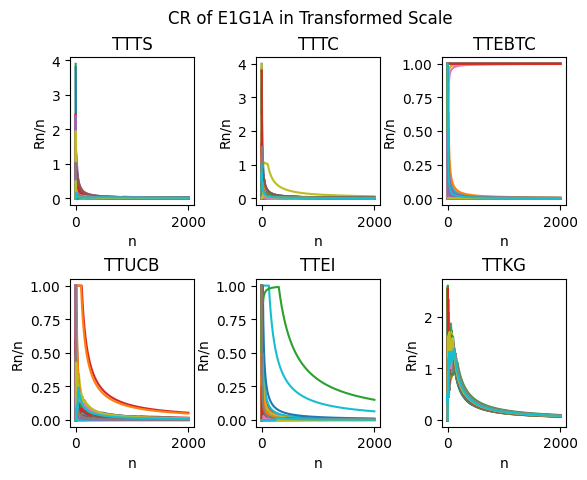
\includegraphics[width=\textwidth]{figures/exp1_cr1.png}
\end{minipage}%
\begin{minipage}{.5\textwidth}
  \centering
  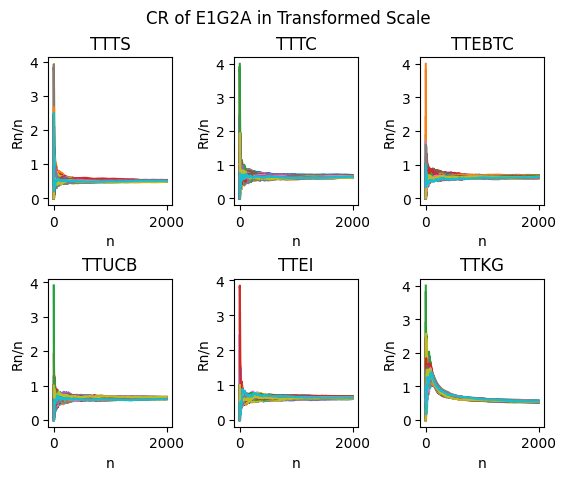
\includegraphics[width=\textwidth]{figures/exp1_cr2.png}
\end{minipage}
\caption{Experiment 1 - Group 1A and 2A Average Cumulative Regret}
\label{figure:exp1_cr}
\end{figure}

In the left graphs, excluding the red outliers in TTEBTC, we observe that most top-one algorithms exhibit a tendency towards greediness. They repetitively select the same leading arm, as evidenced by their nearly zero average cumulative regret (CR) values. Consequently, this behavior results in a large posterior variance for the non-leading arms, thereby prolonging the stopping time.

In contrast, top-two algorithms distribute more pulls among the non-leading arms, as indicated by their non-zero average CR values. This balanced allocation facilitates a more equitable reduction in posterior variance across all arms, leading to a more efficient achievement of the stopping rule.

In the context of the Multi-Armed Bandit problem, this observation underscores the importance of adhering to the recommended arm once the stopping rule has been satisfied. Further exploration beyond this point is futile, as it offers no additional utility.

\subsubsection{High Average Number of Iterations for EI and Failure Rate for EB in Group 1}
In Groups 1A and 1B, EI averaged over 118 iterations to find a solution, while the rest of the algorithms in the group ranged from 12 to 21 iterations. Conversely, EB in Groups 1A and 1B had means of 19.89 and 19.52 iterations, respectively, but suffered from a 55\% and 73\% failure rate. This indicates that while 2000 iterations may not be sufficient to find a solution most of the time, in some instances, EB discovered the best arm very quickly. The histogram below, with a bin size of 50, illustrates this scenario:

\begin{figure}[H] \centering
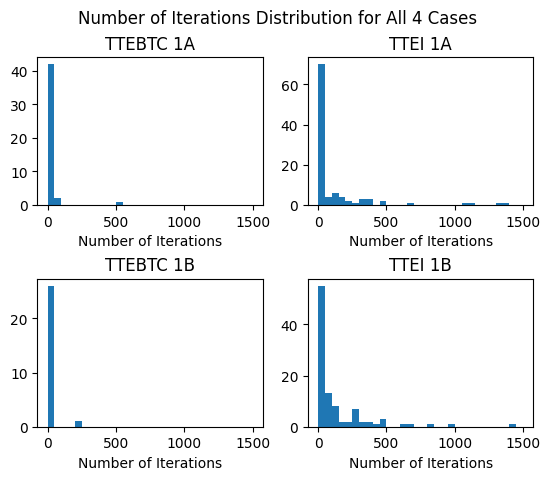
\includegraphics{figures/exp1_itercount.png} 
\caption{Experiment 1 - Group 1 EI and EB Number of Iterations Histogram}
\label{figure:exp1_itercount}
\end{figure}

From the histogram above, we observe that the number of iterations is denser on the left side for most cases. This is because EB had a high failure rate, so many repetitions are not included in the left graphs. With this in mind, we can make an observation: EB had a smaller average number of iterations compared to EI simply because among the repetitions where it did not fail, it performed relatively well. However, the drawback of having such a high failure rate outweighs this advantage. On the other hand, EI had a higher mean yet a 0\% failure rate. The poor performance of these two algorithms can be attributed to the method they employ for selecting the leader $L_n$, both of which can be overly greedy.

In EB, the Empirical Best method is employed, which may suffer from unfortunate initialization and pulls. For instance, in one instance of Group 1A, the arms' empirical means are initialized to $[3.83, 4.36, 1.37, 0.92, 0.54]$. According to the sampling rule in Equation \ref{eq:ttebtc}, it will always select the arm with the highest posterior mean, which is arm $2$ in this case. Although the posterior mean of arm $2$ eventually becomes lower than arm $1$ after a few iterations, another unlucky low-pull reward from arm $1$ causes its posterior mean to drop to $3.56$. From that point onward, the algorithm exclusively pulls arm $2$ for the remaining iterations, failing to pass the stopping rule due to insufficient evidence to confirm or refute its status as the best arm.

In contrast, EI aims to identify the arm with the greatest potential for improvement. While it is not susceptible to unlucky initializations, it can become excessively greedy once it identifies a particular arm as the best candidate. For instance, in one instance of Group 1B, the algorithm ran for 1445 iterations because it allocated the majority of its pulls to arm $1$, exploring arm $2$ only six times. Upon reaching the stopping rule and examining the final posterior distribution, arm $2$ exhibited a posterior variance of 0.17 and a posterior mean of 1.33, significantly higher than its actual mean of 0.8. This greedy behavior substantially prolongs the stopping time by over 100 iterations.

\subsubsection{Large Difference in the Average Number of Iterations of TTTS and T3C in Group 1A}
In Group 1A, there was a significant difference in the mean number of iterations for the top-one versions of TS (17.15) and TTTC (12.74), despite both algorithms employing the exact same leader sampling rule. The reason for this difference can be deduced easily, as both algorithms utilize a purely random sampling rule, involving selecting the best sample from the posterior distribution. Consequently, when there is poor initialization, the posterior sampling becomes less accurate, leading to a cascading effect of pulling the non-optimal arm more times than necessary.

For instance, in one instance of Group 1A TS run, arms $1$ and $2$ were initialized to 4.32 and 5.62, respectively, despite the actual mean of arm $1$ being higher. Consequently, during posterior sampling from the distribution $\Pi_n$ in the subsequent iterations, arm $2$ obtained the highest $v_{i,n}$ value most of the time, causing the algorithm to repeatedly select it as $L_n$ and waste several iterations. Therefore, we can conclude that the difference in the average number of iterations is entirely due to the randomization seed.

\subsubsection{Conclusion}
From this experiment, we can confidently assert that the top-two versions of all algorithms outperform their top-one counterparts. This conclusion is supported by the lower average number of iterations, lower failure rate, and greater robustness to random occurrences exhibited by the top-two versions. there are some intriguing observations that may provide valuable insights for the analysis in the next experiment.

The comparison of the average number of iterations clearly highlights the superiority of top-two algorithms over their top-one counterparts across all cases. This discrepancy can be attributed to the inherent greediness of the top-one algorithms in arm selection, which results in only a marginal reduction in the posterior variance of non-optimal arms. While this approach may seem reasonable at first glance, it ultimately leads to a less efficient pathway towards achieving the stopping rule.

Additionally, specific shortcomings observed in top-one algorithms, such as EI and EB failing to deliver prompt solutions, were addressed and rectified in the top-two versions. EI required a significantly higher number of iterations to reach the stopping rule, while EB failed in the majority of repetitions. These issues were mitigated in the top-two versions by introducing a second candidate to the leader, facilitating a more explorative approach and addressing the problem of shortsightedness.

Lastly, the effect of purely random sampling rules in top-one algorithms, as seen in the disparate performance of TS and T3C despite their identical nature, underscores the need for further investigation. This discrepancy arises from the cascading effect of randomization in leader sampling. In the next experiment, we shall explore whether this effect is successfully mitigated by the addition of challenger sampling rules.


\subsection{Experiment 2: Effect of True Means Separation}
Now that we've established that the top-two modification has significantly enhanced the top-one algorithms, we will proceed to compare how each of the top-two algorithms adapts to different problem settings. In this second experiment, we will focus on the distance between the true means as the main independent variable. Below are the parameters for this experiment:

\begin{table*}[hbt!]
\centering
\begin{tabular}{lccc}
\hline
Parameter & Group 1 & Group 2 & Group 3 \\
\hline
Distribution & \multicolumn{3}{c}{Normal} \\
True Arm $\mu$ & [5,3.3,3.2,3.1,3] & [5,4,3,2,1] & [3,2.5,2,1.5,1] \\
True Arm $\sigma^2$ & \multicolumn{3}{c}{1} \\
Parameters & \multicolumn{3}{c}{None} \\
Algorithm Type & \multicolumn{3}{c}{Top Two} \\
Algorithm & \multicolumn{3}{c}{All} \\
Confidence Level & \multicolumn{3}{c}{0.9999} \\
\hline
\end{tabular}
\caption{Experiment 2 - Parameters}
\label{table:exp2_param}
\end{table*}

Unlike before, we only have three experiment groups: Group 1 for the moderately-separated set ($[5,3.3,3.2,3.1,3]$), Group 2 for the set with a mean distance of 1 ($[5,4,3,2,1]$), and Group 3 for the set with a mean distance of 0.5 ($[3,2.5,2,1.5,1]$). By gradually increasing the difficulty, we aim to gain a clearer understanding of the capabilities of these algorithms in significantly more complex scenarios.

First, we will evaluate the average number of iterations required to reach the 0.9999 confidence level for each of the groups, along with their corresponding failure rates (if any):

\begin{table*}[hbt!]
\centering
\begin{tabular}{lccc}
\hline
Algo & Group 1 & Group 2 & Group 3 \\
\hline
TTTS & 37.68 & 63.19 & 206.57 \\
TTTC & 36.88 & 61.37 & 229.15 \\
TTEBTC & 38.22 & 59.08 & 263.37 \\
TTUCB & 34.95 & 59.09 & 239.3 \\
TTEI & 35.27 & 57.97 & 237.17 \\
TTKG & 45.31 & 74.81 & 286.75 \\
\hline
\end{tabular}
\caption{Experiment 2 - Average Number of Iterations and Failure Rate (if non-0)}
\label{table:exp2_iter}
\end{table*}

Among the top-two algorithms, none of them failed to converge to a solution in under 2000 iterations, despite the increased difficulty of the problem. As expected, the average number of iterations required to achieve the stopping rule increased exponentially as the true means became closer together. Now, let's delve into the intra-group comparison between each of the algorithms to discern their strengths and weaknesses.

Upon initial inspection, there weren't any significant anomalies in the results, unlike the first experiment. All of the algorithms performed relatively well, with some converging faster than others in certain cases, and vice versa. However, three general trends emerge across the three groups:

\begin{enumerate}
\item TTKG consistently performed the worst among all three groups by a large margin.
\item TTEI and TTUCB consistently delivered solutions at a quick and stable rate across all three groups.
\item TTTS and TTTC performed moderately in the first two groups, but notably outperformed all the other algorithms in Group 3 by a considerable margin.
\end{enumerate}

\subsubsection{A poor performance by TTKG in all 3 groups}
The most noticeable occurrence is TTKG being the worst performer in all three groups in terms of average number of iterations. In Groups 1 and 2, it took 18\% longer than the next worst algorithms, while in Group 3, it was 8\% longer. To deduce the reason behind this poor performance, let's examine the cumulative regret graph on a transformed scale ($\frac{R_n}{n}$). For simplicity, we will only show the graph for Group 1, as the patterns are very similar in the other two groups:

\begin{figure}[H] \centering
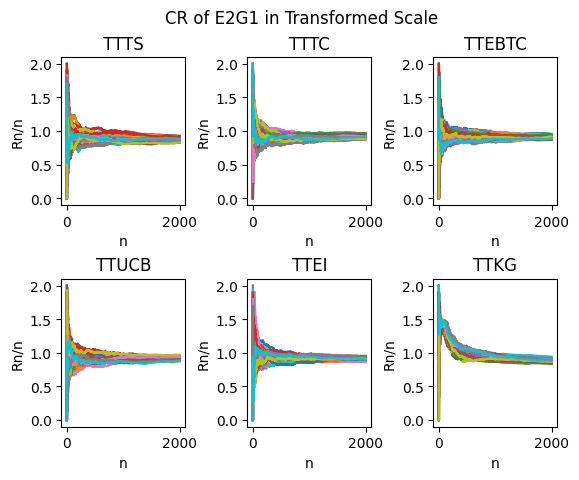
\includegraphics{figures/exp2_cr.png} 
\caption{Experiment 2 - Group 1 Average Cumulative Regret}
\label{figure:exp2_cr}
\end{figure}

In the initial values of TTKG from the graph above, we observe that its average cumulative regret is significantly higher compared to the other algorithms. TTKG converges to 1.5 at a relatively low value of $n$ before swiftly dropping to 1. Then, it gradually decreases at a less noticeable pace. This behavior starkly contrasts with the other five algorithms, which promptly converge to 1 before experiencing the same slow decline over subsequent iterations.

The high average cumulative regret indicates that, in the early iterations, TTKG allocates an excessive number of pulls to non-optimal arms with a mean difference of around 1.5 from the true optimal arm. Conversely, the other algorithms quickly prioritize only the most promising arms. This behavior aligns with the exploratory nature of TTKG, which we previously identified. In the first experiment, this flaw remained hidden as the confidence level was set at a very low value (0.95). Consequently, minimal exploitation was less penalized, as the stopping rule could be achieved even with 0 iterations on arm 1 and a fortunate initialization of the arms.

\subsubsection{A fast and stable performance by TTEI and TTUCB in all 3 groups}
Another noteworthy result is the consistent and efficient performance of TTEI and TTUCB, which delivered solutions with the fewest average number of iterations in the first two groups, around 35 and 58.5, respectively. Even in Group 3, where they were not the fastest, TTEI and TTUCB still performed relatively well, trailing slightly behind TTTS and TTTC. This outcome is surprising given that in Experiment 1, the original EI algorithm performed significantly worse than most other top-one algorithms due to its excessive greediness.

The notable enhancement in EI's performance following the integration of the challenger into the arm sampling process suggests a reduction in its greediness, leading to a considerable improvement in its exploratory rate. By revisiting the sampling rule in Equation \ref{eq:ttei}, which dictates selecting the leader based on the expected improvement over the current best-sampled arm and subsequently choosing the challenger based on its expected improvement over the leader, we can deduce that this modification enables the inclusion of some of the lesser arms as potential candidates. Consequently, it achieves a finer balance between exploitation and exploration, a pivotal factor contributing to the algorithm's significant performance boost.

In contrast, the top-one UCB algorithm, a well-established approach for Best Arm Identification, performed relatively well in Experiment 1 and continued to excel in its top-two version in Experiment 2, even with a higher confidence level. This success underscores the effectiveness of both the algorithm's leader and challenger sampling rules in balancing exploitation and exploration. Examining the sampling rule in Equation \ref{eq:ttucb}, it becomes evident that the leader sampling rule takes into account both exploitation (represented by the $\mu_{i,n}$ term) and exploration (uncertainty term). Similarly, the challenger, leveraging the concept of transportation costs, also considers these two factors.

\subsubsection{A moderate performance by TTTS and T3C in Groups 1 and 2, but an extremely fast solution in Group 3}
In the first two groups, TTTS and T3C performed moderately well, trailing behind TTUCB and TTEI by a small margin. However, in the most challenging problem-setting, they surged ahead to become the two fastest algorithms, with TTTS finishing an average of 31 iterations faster than TTEI.

Recall that in the first experiment, we identified the significant variation in the performance of the TS and T3C leader sampling rules due to their random nature. This randomness could cascade, leading to considerable variation in outcomes. To mitigate this variation, we introduced a top-two modification by incorporating a second random challenger sampling rule for TTTS and a deterministic one for T3C. To ascertain the success of this modification and determine whether the random nature of these algorithms influenced this reversal in performance, we conducted the Group 3 setting using three other distinct seeds. Here are the new results:

\begin{table*}[hbt!]
\centering
\begin{tabular}{lcccc}
\hline
Algo & Original Seed & Seed 1 & Seed 2 & Seed 3 \\
\hline
TTTS & 206.57 & 240.34 & 209.35 & 232.91 \\
TTTC & 229.15 & 239.64 & 242.72 & 232.33 \\
TTEBTC & 263.37 & 251.48 & 248.21 & 241.10 \\
TTUCB & 239.3 & 214.76 & 231.67 & 241.09 \\
TTEI & 237.17 & 232.26 & 228.93 & 226.53 \\
TTKG & 286.75 & 293.57 & 289.89 & 283.78 \\
\hline
\end{tabular}
\caption{Experiment 2 - G3 Average Number of Iterations and Failure Rate (if non-0)}
\label{table:exp2_iter_g3}
\end{table*}

From the table, we observe a notable variation for TTTS and T3C, with the difference between the lowest and highest average number of iterations reaching 33.77 for TTTS but only 13.57 for T3C. Moreover, in instances where these two algorithms perform less effectively, they may fall behind either TTEI or TTUCB, indicating that none of these four algorithms are strictly superior to the others.

And now, regarding the success of the top-two modifications and the cause of this reversal in performance, we find that the top-two modification has modestly reduced the variation of T3C by introducing a deterministic challenger that does not rely solely on randomization. However, TTTS remains highly variable, as expected, since it employs another random-based challenger. This underscores the notion that introducing a random-based challenger cannot fully address the issues caused by a random-based leader.

\subsubsection{Conclusion}
In this second experiment, we compared the top-two algorithms to each other and identified instances where certain algorithms outperformed others. However, not all algorithms performed well, and some persistent issues from the top-one versions remained apparent.

In all settings of Experiment 2, TTKG consistently performed poorly, exhibiting the highest average number of iterations. We deduced that the issue stems from its sampling rule nature, which leans towards insufficient exploitation and excessive exploration. These tendencies are penalized more severely at higher confidence levels and when the means are closer together.

Then, on the brighter side of the results, TTEI and TTUCB showcased effective strategies for balancing exploitation and exploration. Despite its suboptimal performance as a top-one algorithm in Experiment 1, EI made significant strides by integrating an exploratory challenger into its previously greedy sampling approach. Similarly, UCB, which already exhibited strong performance as a top-one algorithm, further improved by incorporating a balanced challenger sampling rule alongside its well-defined leader sampling rule.

Finally, we observe a similar randomness effect persisting from Experiment 1 to Experiment 2, resulting in TTTS and T3C outperforming TTEI and TTUCB in Group 3, despite lagging behind them in the first two groups. While the deterministic challenger in T3C has partially mitigated this effect, as evidenced by the lower variation in results, TTTS remains largely unaffected as expected, due to its equally random challenger sampling rule.


\subsection{Experiment 3: Effect of True Common Variance}
Now that we've observed the effects of altering the mean distance between the arms, we'll investigate how the top-two algorithms perform under conditions of increased variance in the reward distributions. In this experiment, the means of the distributions remain constant, but we'll systematically augment the variance, resulting in greater dispersion and less predictable rewards. Below are the parameters defining this experiment:

\begin{table*}[hbt!]
\centering
\begin{tabular}{lccc}
\hline
Parameter & Group 1 & Group 2 & Group 3 \\
\hline
Distribution & \multicolumn{3}{c}{Normal} \\
True Arm $\mu$ & \multicolumn{3}{c}{[5,4,3,2,1]} \\
True Arm $\sigma^2$ & 1 & 2.25 & 5 \\
Parameters & \multicolumn{3}{c}{None} \\
Algorithm Type & \multicolumn{3}{c}{Top Two} \\
Algorithm & \multicolumn{3}{c}{All} \\
Confidence Level & \multicolumn{3}{c}{0.9999} \\
\hline
\end{tabular}
\caption{Experiment 3 - Parameters}
\label{table:exp3_param}
\end{table*}

We have three groups in Experiment 3. Group 1 corresponds to the same setting as Group 2 of Experiment 2, while Group 2 and Group 3 have an increased common variance for all the arms, which are 2.25 and 4 respectively. In other words, we are increasing the standard deviation by 0.5 each time, from 1 to 1.5 and 2.

As usual, for each of the groups, we will assess the average number of iterations required to reach the 0.9999 confidence level alongside their failure rate (if any):

\begin{table*}[hbt!]
\centering
\begin{tabular}{lccc}
\hline
Algo & Group 1 & Group 2 & Group 3 \\
\hline
TTTS & 63.19 & 130.41 & 206.57\\
TTTC & 61.37 & 123.97 & 229.15\\
TTEBTC & 59.08 & 140.15 & 263.37\\
TTUCB & 59.09 & 132.83 & 236.65\\
TTEI & 57.97 & 124.16 & 237.17\\
TTKG & 74.81 & 165.04 & 288.3\\
\hline
\end{tabular}
\caption{Experiment 3 - Average Number of Iterations and Failure Rate (if non-0)}
\label{table:exp3_iter}
\end{table*}

In Experiment 3, across all three scenarios, none of the top-two algorithms failed to converge, and all successfully found a solution in under 300 iterations out of the allocated 2000. And also, Similar trends to those observed in Experiment 2 emerge:
\begin{itemize}
    \item TTKG remains consistently the worst-performing algorithm across all different values of $\sigma^2$
    \item TTEI, TTUCB, TTTS, and T3C consistently emerge as the top-performing algorithms, although there isn't a strict ranking among them.
\end{itemize}

Nevertheless, a new intriguing observation across the three groups has caught our attention:

\begin{enumerate}
    \item The average number of iterations for TTTS, TTTC, TTEBTC, and TTEI in Group 3 is identical to that of Group 3 in Experiment 2, despite the variations in parameters.
\end{enumerate}

\subsubsection{Similar results in Group 3 of Experiments 2 and 3}

First of all, we shall see a recap of the average number of iterations from Group 3 of Experiment 2 and 3:

\begin{table*}[hbt!]
\centering
\begin{tabular}{lcc}
\hline
Algo & Experiment 2 Group 3 & Experiment 3 Group 3 \\
\hline
TTTS & 206.57 & 206.57\\
TTTC & 229.15 & 229.15\\
TTEBTC & 263.37 & 263.37\\
TTUCB & 239.3 & 236.65\\
TTEI & 237.17& 237.17\\
TTKG & 286.75 & 288.3\\
\hline
\end{tabular}
\caption{Experiment 3 - E2 E3 Average Number of Iterations and Failure Rate (if non-0)}
\label{table:exp3_iter_e2e3}
\end{table*}

In the previous experiment, we examined the impact of reducing the distance between each arm while maintaining a constant common variance. In Group 3 of that experiment, we set the separation to 0.5. Conversely, in this experiment, we kept the means constant and altered the variance or spread of the arms' distributions, where in Group 3, we increased the variance to 4 (standard deviation of 2). Surprisingly, we observed identical results in four of the algorithms: TTTS, T3C, TTEBTC, and TTEI, while the other two showed slight variations. 

To understand the reason behind this occurrence, let's first analyze the impact of decreasing the mean separation and increasing the variance. Consider two random variables drawn from distinct Normal distributions, each with different means but sharing the same variance, $X \sim N(\mu_1, \sigma^2)$ and $Y \sim N(\mu_2, \sigma^2)$, where $\mu_1\geq\mu_2$. We want to calculate the probability $P(X \geq Y)$, or equivalently $P(V \geq 0)$, where $V = X-Y$. To compute this, we calculate the distribution of $V$, which is $N(\mu_V, \sigma^2_V)$, where $\mu_V = \mu_1-\mu_2$ and $\sigma^2_V = 2\sigma^2)$. Then, using the cumulative distribution function (CDF) of this new Normal distribution, we can conclude that $P(V \geq 0) = P(Z \geq \frac{0-\mu_V}{\sigma_V}) = P(Z \leq \frac{\mu_V}{\sigma_V})$, where $Z$ is the standard Normal distribution.

From this equation, we observe that the probability of $X$ being greater than $Y$ is solely determined by the ratio $\frac{\mu_V}{\sigma_V} = \frac{\mu_V}{\sqrt{2}\sigma} \approx \frac{\mu_V}{\sigma}$, with the 2 variables $\mu_V$ and $\sigma$ being inversely proportional. Hence, if we increase the mean separation by a constant $k$, we can offset its effects by also increasing the standard deviation by $k$ as well. For example, in Experiment 2, we have $\mu_V = 0.5$ and $\sigma_V = 1$, while in Experiment 3, we have $\mu_V = 1$ and $\sigma_V = 2$. It is evident that $\frac{\mu_V}{\sigma} = 0.5$ in both cases, indicating that the probability of arm $i$ being greater than arm $i+1$ for $i\in \{1,2,...n-1\}$ remains the same in both experiments.

Given this property, we can comprehend why four of the algorithms yielded identical results in both experiments, while TTUCB and TTKG did not. The sampling rules of TTTS, T3C, TTEBTC, and TTEI rely entirely on assumptions based on the Normal distribution, such as empirical sampling for TTTS and T3C, transportation cost estimation for T3C and TTEBTC, empirical best sampling for TTEBTC, and expected improvement calculation for TTEI. This alignment with the property explained above led to consistent results. 

On the other hand, neither of the other two algorithms employed a purely Normal sampling rule. TTKG, although utilizing a similar assumption to TTEI, incorporates a one-step-ahead variance calculation, which could introduce inaccuracies. Additionally, TTUCB adopts the negative branch of the Lambert W function as its leader sampling rule, deviating from the expected outcome due to its departure from the Normal distribution-based approach.

\subsubsection{Conclusion}
In Experiment 3, we observed familiar trends that echoed those seen in Experiment 2, including the consistent performance of certain algorithms. Additionally, we noticed an intriguing correlation between increasing the mean separation and decreasing the variance of set $A$.

In Group 3 of Experiments 2 and 3, we obtained identical average numbers of iterations for TTTS, T3C, TTEBTC, and TTEI when we halved the mean distance and doubled the standard deviation. This phenomenon can be attributed to the ratio $\frac{\mu_V}{\sigma}$, which entirely governs the probability $P(X-Y \geq 0)$, where $X$ and $Y$ represent the rewards of arm $i$ and arm $i+1$ respectively. This consistency arises because these four algorithms solely rely on pure Normal distribution-based leader and challenger sampling rules. Meanwhile, TTKG and TTUCB, which employ partial Normal sampling rules, did not exhibit the same behavior.


\subsection{Experiment 4: Effect of True Distribution Type}

In the previous three experiments, our focus was primarily on assessing the performance of our algorithms when dealing with arms drawn from Normal distributions. Now, for our final experiment, we'll explore how these algorithms fare when confronted with arms drawn from Gamma and Beta distributions. In this scenario, we'll maintain the same mean and variance, only adjusting the shape and rate parameters, denoted by $\alpha$ and $b$, respectively. Below are the parameters defining this experiment:

\begin{table*}[hbt!]
\centering
\begin{tabular}{lcccccc}
\hline
Parameter & Group 1 & Group 2 & Group 3 & Group 4 & Group 5 & Group 6\\
\hline
Distribution & Normal & Gamma & Gamma & Beta & Beta & Beta \\
True Arm $\mu$ & \multicolumn{6}{c}{[5,4.5,4,3.5,3]} \\
True Arm $\sigma^2$ & \multicolumn{6}{c}{1} \\
Parameters & None & 3 & 1.5 & (2,2) & (2,5) & (0.9,0.9) \\
Algorithm Type & \multicolumn{6}{c}{Top Two} \\
Algorithm & \multicolumn{6}{c}{All} \\
Confidence Level & \multicolumn{6}{c}{0.9999} \\
\hline
\end{tabular}
\caption{Experiment 4 - Parameters}
\label{table:exp4_param}
\end{table*}

In Experiment 4, we've divided the study into 6 groups. Group 1 pertains to the Normal distribution, while Groups 2 to 3 are associated with the Gamma distribution, and Groups 4 to 6 correspond to the Beta distribution. Across all groups, the means and variances will remain consistent at [5, 4.5, 4, 3.5, 3], and 1, respectively. However, the $\alpha$ and $b$ parameters will vary to serve as the primary independent variables for the Gamma and Beta Groups. These parameters are carefully chosen to ensure that each group displays distinct skewness, kurtosis, or overall shape, while preserving consistent mean and variance for fair comparison across the groups.

To better visualize these differences, we'll plot scaled and shifted probability density function for each distribution:

\begin{figure}[H] \centering
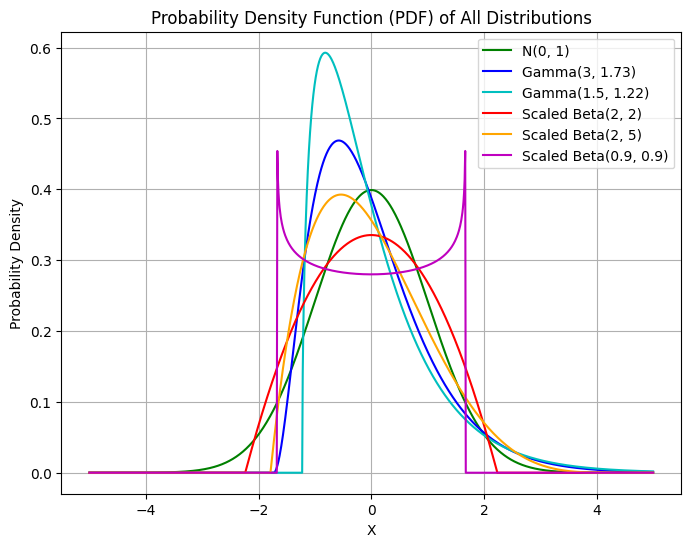
\includegraphics[width=\textwidth]{figures/exp4_pdf.png} 
\caption{Experiment 4 - Group 4 Distribution PDFs}
\label{figure:exp4_pdf}
\end{figure}

In Group 2 (dark blue), we set the $\alpha$ parameter of the Gamma distribution to be 3 and then compute $b$ to be 1.73. Moving to Group 3 (cyan), we increase the difficulty by halving the $\alpha$ of the distribution and adjusting $b$ accordingly to $1.22$. This adjustment aims to enhance the skewness of the distribution while maintaining the mean and variance. Recall that the skewness of a Gamma distribution can be calculated by the formula $\frac{2}{\sqrt{\alpha}}$, indicating that the PDF becomes less symmetrical as we decrease $\alpha$.


In Groups 3-5, we further manipulate the shape of the Beta distribution, introducing greater variability compared to the Gamma distribution. Group 4 (red) showcases a symmetric $\mathrm{Beta}(2,2)$ distribution characterized by heavier tails and a more pronounced peak, resulting in higher kurtosis (leptokurtic) compared to the Normal Distribution. Moving to Group 5 (orange), we introduce skewness to this distribution. Lastly, Group 6 (magenta) presents a symmetric distribution with modes at both ends. This modification doesn't skew the probability density function but rather alters the overall shape of the distribution to resemble a Uniform distribution that is pushed down in the middle, resulting in a more convex shape.

Now, having understood the overall shapes and distributions, we're interested in analyzing the performance of the algorithms in terms of the average number of iterations required to reach the 0.9999 confidence level, as well as their failure rate (if any):

\begin{table*}[hbt!]
\centering
\begin{tabular}{lcccccc}
\hline
Algo & Group 1 & Group 2 & Group 3 & Group 4 & Group 5 & Group 6 \\
\hline
TTTS & 206.57 & 219.39 & 208.69 & 226.64 & 216.9 & 202.11 \\
TTTC & 229.15 & 243.46 & 231.91 & 243.42 & 232.08 & 239.71 \\
TTEBTC & 263.37 & 241.14 & 254.46 & 229.94 & 249.68 & 243.62 \\
TTUCB & 239.30 & 229.95 & 221.88 & 241.31 & 227.98 & 222.70 \\
TTEI & 237.17 & 237.18 & 236.82 & 226.54 & 230.64 & 232.23 \\
TTKG & 286.75 & 305.42 & 294.18 & 259.97 & 292.55 & 311.23 \\
\hline
\end{tabular}
\caption{Experiment 4 - Average Number of Iterations and Failure Rate (if non-0)}
\label{table:exp4_iter}
\end{table*}

Across the algorithms, we observe similar trends in the performance of TTKG as well as the top 4 algorithms. However, despite the extreme modifications that were expected to challenge the algorithms, the results did not align with our expectations:

\begin{enumerate}
    \item Surprisingly, the average number of iterations in these 5 Groups is not necessarily higher than that of Group 1's Normal distribution, despite the significant alterations to the distributions.
\end{enumerate}

\subsubsection{Solution on Normal distribution is not strictly faster than the others}
The most striking observation in this experiment is the lower average number of iterations required to solve some of the non-Normal distributions compared to the Normal distribution, despite our underlying Normal prior and posterior distributions.

Initially, this might seem counter intuitive, as a Normal distribution inherently cannot perfectly match the shape of a Beta or Gamma distribution. However, it's essential to remember that our posterior distribution aims to parameterize the current mean estimate $\mu_{i,n}$ to converge towards the true means $\mu_i$ as the number of pulls increases, while simultaneously reducing the uncertainty $\sigma^2$ towards 0. It's not attempting to precisely replicate the exact shape of the true distributions, which would indeed be impossible.

Furthermore, in our update equations (\ref{eq:miu_update}) and (\ref{eq:sigma_update}), we weight the reward based on its variance and the current $\mu_{i,n}$ estimation according to its uncertainty. This weighting mechanism is beneficial, especially in the case of non-Normal distributions where some probability density functions exhibit high kurtosis. In such distributions, outliers are more likely, which could potentially impact the calculation of $\mu_{i,n+1}$. The weighted sum helps mitigate the influence of short-term rewards, contributing to the overall effectiveness of the algorithm.

\subsubsection{Conclusion}
In this experiment, we sought to challenge the six algorithms with five non-Normal scenarios, anticipating potential struggles due to the unfamiliar nature of these distributions. However, we observed consistent trends in the performance of TTKG and the four faster algorithms across these scenarios. And more surprisingly, they managed to solve these non-Normal distributions in a similar number of iterations or even faster compared to the Normal distribution. This unexpected outcome highlights the robustness of our posterior distribution updating rule. It implies that algorithms utilizing this rule are equipped to handle various error distributions effectively. This robustness is a crucial finding for future research endeavors with broader distributions.



\section{Conclusion}
\subsection{Summary}
In this thesis, we embarked on a comprehensive exploration of multi-armed bandit algorithms, delving deep into the building blocks that form them as well as the sampling rules that describe their choice of leader and challenger. Additionally, we attempted to compute the rate of posterior convergence in terms of $\Gamma_\beta^*$ to demonstrate the optimality property of using any particular $\beta$ value for the top-two algorithms. In the process, we also established that the arms converge to asymptotically optimal proportions.

Then, through a series of experiments, we scrutinized the efficacy of both top-one and top-two algorithms under diverse conditions, shedding light on their strengths, weaknesses, and underlying mechanisms, while evaluating them based on three important metrics.

Our investigation commenced with a comparison between top-one and top-two algorithms in Experiment 1. Here, we observed a marked improvement in performance with the adoption of the top-two approach. This enhancement stemmed from the reduced greediness and heightened exploratory rate facilitated by the incorporation of challengers in the arm sampling process. Algorithms such as Expected Improvement (EI) and Upper Confidence Bound (UCB) demonstrated a more balanced exploitation-exploration trade-off, resulting in substantial performance gains. Thompson Sampling, meanwhile, exhibited a high level of randomness in its leader sampling rule, mirroring that of top-one T3C, as they are compeletely identical.

Experiment 2 extended our analysis to challenging problem settings, namely the increase in the mean distance between the arms. Notably, TTKG appeared to perform sub-optimally compared to other algorithms. Furthermore, the addition of challengers mitigated the adverse effects of randomness in leader sampling, particularly evident in T3C but less so in TTTS. However, despite the increased difficulty and variations in solving speed, top-two algorithms consistently delivered solutions within a small disparity in performance and a 0\% failure rate, indicating the success of the modifications.

Further exploration in Experiment 3 focused on the impact of increasing variance in reward distributions. Similar trends from Experiments 1 and 2 reoccurred, and it was also shown that for algorithms which highly rely on Normal-based sampling rules, namely TTTS, T3C, TTEBTC, and TTEI, the same result will appear should the ratio $\frac{\mu_V}{\sigma}$ be identical.

Finally, Experiment 4 delved into the performance of algorithms across different true underlying distributions of the arms. Surprisingly, top-two algorithms exhibited resilience to non-Normal distributions, outperforming their performance even in the face of challenging distributions such as Beta and Gamma with odd shapes. This resilience underscored the robustness of the posterior distribution updating rule employed by these algorithms, which prioritizes convergence to true means over exact distribution fitting.


\subsection{Implications of Practical Applications}
The implications of our research findings extend, not only in this problem scope, but also to various practical applications in fields, such as online advertising, healthcare, finance, and more. 

In online advertising, for instance, where advertisers face the challenge of optimizing ad placement to maximize click-through rates, our insights into bandit algorithms can help in efficiently allocating resources to different ad variants while simultaneously exploring new strategies to improve performance. 

Similarly, in healthcare, where clinical trials aim to identify the most effective treatments, bandit algorithms can assist in dynamically allocating patients to different treatment arms based on evolving evidence, leading to more efficient and personalized healthcare interventions.

Moreover, in financial markets, where traders seek to optimize investment strategies while managing risk, bandit algorithms can aid in portfolio optimization by dynamically allocating capital to different assets based on real-time market conditions. By striking a balance between exploiting known profitable opportunities and exploring new investment possibilities, these algorithms can help investors achieve better returns while mitigating risks. 

And lastly, in recommendation systems used in e-commerce platforms and streaming services, bandit algorithms can enhance user experience by intelligently selecting and presenting content tailored to individual preferences, thereby increasing user engagement and satisfaction.

Overall, the practical applications of bandit algorithms are diverse and far-reaching, offering valuable insights and tools for decision-making in various domains. By leveraging the insights gained from our research, practitioners can develop more efficient and adaptive systems that better meet the evolving needs of users and stakeholders in a wide range of real-world applications.


\subsection{Future Research}
Future research in the field of bandit algorithms holds promising avenues for further exploration and innovation. One direction for future investigation is the development of advanced algorithms that can effectively handle more complex decision-making scenarios, such as those involving multiple competing objectives or uncertain environments with non-stationary dynamics. By incorporating sophisticated learning mechanisms and adaptive strategies, future bandit algorithms could potentially achieve better performance and robustness in such challenging settings.

Another area of interest for future research is the exploration of novel applications and domains where bandit algorithms can offer significant benefits. For example, in the context of autonomous vehicles, bandit algorithms could be employed to optimize driving strategies in real-time, considering factors such as traffic conditions, weather, and passenger preferences. Similarly, in healthcare, bandit algorithms could be used to optimize treatment plans for individual patients based on personalized medical data, leading to more effective and efficient healthcare delivery.

Furthermore, future research could focus on enhancing the interpretability and transparency of bandit algorithms, particularly in high-stakes applications where human oversight and understanding are crucial. By developing methods for explaining and visualizing the decision-making process of bandit algorithms, researchers can improve trust and accountability in automated systems, enabling more responsible deployment in real-world settings. Overall, future research in bandit algorithms holds great potential to advance our understanding of decision-making under uncertainty and to drive innovation in a wide range of practical applications.


\subsection{Final Remarks}
In short, this thesis provides valuable insights into the efficacy of top-one and top-two bandit algorithms in the Best Arm Identification problem, which can arguably be generalized to many other dynamic decision-making tasks. The findings underscore the importance of balancing exploitation and exploration, as well as the robustness to unknown true distributions, with top-two approaches emerging as a promising avenue for future research. As we continue to explore complex decision-making problems, the lessons learned from this thesis will undoubtedly inform the development of more robust and efficient bandit algorithms in diverse real-world applications.



\newpage
%\setcitestyle{round,aysep={},yysep={;}}
\bibliography{bibliography}
\bibliographystyle{plainnat}

% Add the References to the table of contents.
\addcontentsline{toc}{section}{References}

\end{document}
